\documentclass[a4paper, 12pt]{article}%тип документа

%%%Библиотеки
	%\usepackage[warn]{mathtext}	
	\usepackage[T2A]{fontenc} % кодировка
	\usepackage[utf8]{inputenc} % кодировка исходного текста
	\usepackage[english,russian]{babel} % локализация и переносы
	\usepackage{caption}
	\usepackage{listings}
	\usepackage{amsmath,amsfonts,amssymb,amsthm,mathtools}
	\usepackage{wasysym}
	\usepackage{graphicx}%Вставка картинок правильная
	\usepackage{float}%"Плавающие" картинки
	\usepackage{wrapfig}%Обтекание фигур (таблиц, картинок и прочего)
	\usepackage{fancyhdr} %загрузим пакет
	\usepackage{lscape}
	\usepackage{xcolor}
	\usepackage[normalem]{ulem}
	\usepackage{hyperref}

%%%Конец библиотек




%%%Настройка ссылок
	\hypersetup
	{
		colorlinks=true,
		linkcolor=blue,
		filecolor=magenta,
		urlcolor=blue
	}
%%%Конец настройки ссылок


%%%Настройка колонтитулы
	\pagestyle{fancy}
	\fancyhead{}
	\fancyhead[L]{Лабораторная работа}
	\fancyhead[R]{Талашкевич Даниил, группа Б01-009}
	\fancyfoot[C]{\thepage}
%%%конец настройки колонтитулы



							\begin{document}
						%%%%Начало документа%%%%


%%%Начало титульника
\begin{titlepage}

	\newpage
	\begin{center}
		\normalsize Московский физико-технический институт \\(госудраственный 			университет)
	\end{center}

	\vspace{6em}

	\begin{center}
		\Large Лабораторная работа по электричеству\\
	\end{center}

	\vspace{1em}

	\begin{center}
		\large \textbf{Измерение магнитного поля Земли [3.1.3]}
	\end{center}

	\vspace{2em}

	\begin{center}
		\large Талашкевич Даниил Александрович\\
		Группа Б01-009
	\end{center}

	\vspace{\fill}

	\begin{center}
	Долгопрудный \\2021
	\end{center}
	
\end{titlepage}
%%%Конец Титульника



%%%Настройка оглавления и нумерации страниц
	\thispagestyle{empty}
	\newpage
	\tableofcontents
	\newpage
	\setcounter{page}{1}
%%%Настройка оглавления и нумерации страниц


					%%%%%%Начало работы с текстом%%%%%%

\textbf{Цель работы:} исследовать свойства постоянных неодимовых магнитов; измерить с их помощью горизонтальную и вертикальную составляющие индукции магнитного поля Земли и магнитное наклонение. \\

\textbf{Используемое оборудование:} неодимовые магниты; тонкая нить для изготовления крутильного маятника; медная проволока; электронные весы; секундомер; измеритель магнитной индукции; штангенциркуль; брусок, линейка и штатив из немагнитных материалов; набор гирь и разновесов.

\section{Теоретическое введение}

Магнитное поле точечного диполя с магнитным моментом $\textbf{m} = \textbf{S}I$ определяется по формуле, аналогичной формуле для поля элементарного электрического диполя:

\begin{equation}
    \textbf{B}_{\text{дип}} = \frac{\mu_0}{4 \pi} \left( \frac{3(\textbf{m} \cdot \textbf{r})\textbf{r}}{r^5} - \frac{\textbf{m}}{r^3}  \right)
\end{equation}

При этом сила, действующая на диполь, равна

\begin{equation}
    \textbf{F} = (\textbf{m} \cdot \triangledown ) \textbf{B}
\end{equation}

А момент силы равен

\begin{equation}
    \textbf{M} = [ \textbf{m} \times \textbf{B}]
\end{equation}

В частном случае, когда моменты двух небольших магнитов направлены вдоль соединяющей их прямой, сила их взаимодействия равна

\begin{equation}
    F = - \frac{6 m_1 m_2}{r^4}
\end{equation}

Если магнитные моменты направлены перпендикулярно соединяющей их прямой, то

\begin{equation}
    F = \frac{3 m_1 m_2}{r^4}
\end{equation}

\section{Экспериментальное оборудование и методика измерений}

\subsection{Определение магнитного момента магнитных шариков}

\subsubsection{Метод 1}

Величину магнитного момента $m$ двух одинаковых шариков можно рассчитать, зная их массу $M$ и определив максимальное расстояние $r_{max}$, на котором они ещё удерживают друг друга в поле тяжести (см. рис.). Из формулы для взаимодействия диполей имеем

\begin{equation}
    m = \sqrt{\frac{Mgr^4_{max}}{6}}
\end{equation}

Таким образом с помощью измеренного магнитного момента шарика можно измерить индукцию магнитного поля

%\begin{figure}[h]
%    \centering
%    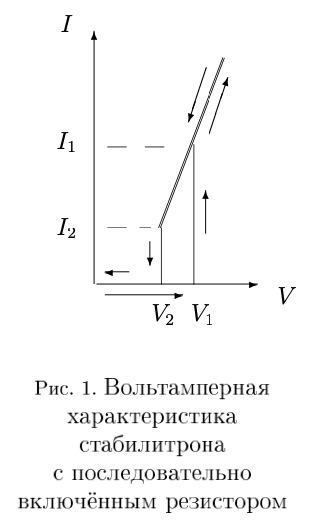
\includegraphics[width = 5 cm]{images/1.png}
%    \caption{Измерение магнитных моментов шариков}
%    \label{msh1}
%\end{figure}

\subsubsection{Метод 2}

Величину магнитного момента шариков можно определить также по силе их сцепления. Она определяется как сила, необходимая для разрыва двух сцепившихся магнитных шариков. Сила сцепления максимальна, если шары соединяются своими противоположными полюсами (магнитные моменты сонаправлены).

Максимальную силу сцепления можно определить по весу магнитной цепочки, которую способен удержать самый верхний магнитный шарик. При этом для расчёта прочности цепочки достаточно учитывать силу взаимодействия верхнего шара с 3–4 ближайшими соседями.

\begin{equation}
    F = \frac{3m^2}{8R^4} \left( 1 + \frac{1}{2^4} + \frac{1}{3^4} + ...\right) = 1,08 \cdot \frac{3m^2}{8R^4}
\end{equation}

\subsection{Измерение горизонтальной составляющей индукции магнитного поля Земли}

Магнитное поле Земли можно измерить по периоду крутильных колебаний «магнитной стрелки» вокруг вертикальной оси.

«Магнитная стрелка» образована сцепленными друг с другом $n$ намагниченными шариками. Для крепления нити в работе используется штатив, изготовленный из немагнитного материала. Магнитные моменты всех шариков направлены в одну сторону вдоль оси «стрелки». При отклонении стрелки на угол $\theta$ от равновесного положения в горизонтальной плоскости возникают крутильные колебания вокруг вертикальной оси, проходящей через середину стрелки.

%\begin{figure}[h]
%    \centering
%    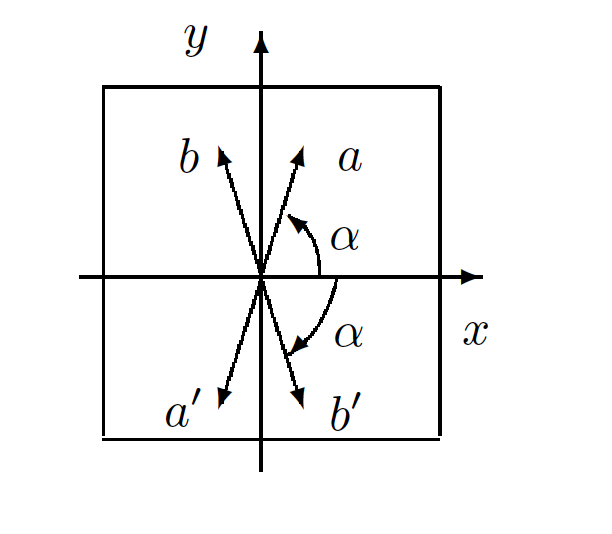
\includegraphics[width = 6 cm]{images/2.png}
%    \caption{ Крутильный маятник во внешнем магнитном поле}
%    \label{sh1}
%\end{figure}

\begin{equation}
    M = -m_n B_{||} \sin{\theta} \Rightarrow J_n \ddot{\theta} + m_n B_{||} \theta = 0 \Rightarrow T = 2 \pi \sqrt{\frac{J_n}{m_n B_{||}}}
\end{equation}

\begin{equation}
    T = 2 \pi \sqrt{\frac{J_n}{m_n B_{||}}} = 2 \pi \sqrt{\frac{n^3 M R^2}{12m_n B_{||}}} \Rightarrow T = 2 \pi \sqrt{\frac{M R^2}{3 m B_{||}}} n
\end{equation}

\subsection{Измерение вертикальной составляющей индукции магнитного поля Земли. Магнитное наклонение}

Для измерения вертикальной составляющей вектора индукции поля Земли используется та же установка, что и для измерения горизонтальной составляющей с тем лишь отличием, что подвешенная магнитная «стрелка» закрепляется на нити в одной точке. В этом случае стрелка, составленная из чётного числа одинаковых шариков и подвешенная за середину, расположится не горизонтально, а под некоторым углом к горизонту.

Это связано с тем, что вектор $\textbf{B}$ индукции магнитного поля Земли не горизонтален, а образует с горизонтом
некоторый угол $\beta$, зависящий от географической широты $\phi$ места, где проводится опыт. Величина угла $\beta$ называется магнитным наклонением.

%\begin{figure}[h]
%    \centering
%    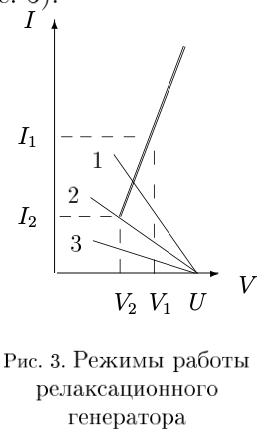
\includegraphics[width = 10 cm]{images/3.png}
%    \caption{Измерение вертикальной составляющей поля и магнитного наклонения}
%    \label{way3}
%\end{figure}

\begin{equation}
    M_n = m B_{\perp} n
\end{equation}

\end{document}
